\documentclass[tikz,border=10pt]{standalone}
\usepackage{pgfplots}
\pgfplotsset{compat=1.16}

\begin{document}
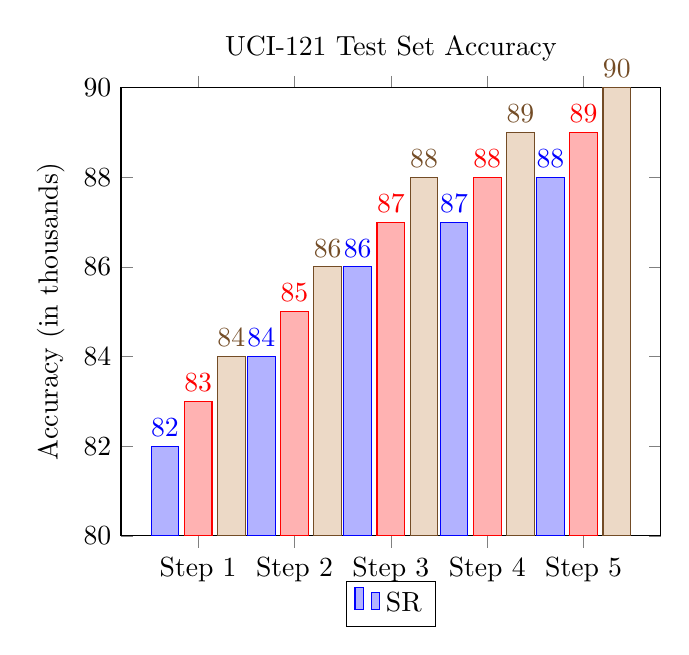
\begin{tikzpicture}
    \begin{axis}[
        ybar,
        symbolic x coords={Step 1, Step 2, Step 3, Step 4, Step 5},
        xtick=data,
        nodes near coords,
        ylabel={Accuracy (in thousands)},
        title={UCI-121 Test Set Accuracy},
        ymin=80,
        ymax=90,
        enlarge x limits=0.2,
        legend style={at={(0.5,-0.1)}, anchor=north}
    ]
        \addplot coordinates {(Step 1, 82) (Step 2, 84) (Step 3, 86) (Step 4, 87) (Step 5, 88)};
        \legend{SVE};
        
        \addplot coordinates {(Step 1, 83) (Step 2, 85) (Step 3, 87) (Step 4, 88) (Step 5, 89)};
        \legend{ENT};
        
        \addplot coordinates {(Step 1, 84) (Step 2, 86) (Step 3, 88) (Step 4, 89) (Step 5, 90)};
        \legend{SR};
    \end{axis}
\end{tikzpicture}
\end{document}